\section{Notation for probabilistisk robotstyring}
Da det er ønskværdigt at kunne give en præcis beskrivelse af robottens positur, dvs. dens position og retning, vil dette afsnit kort introducere den nødvendige notation, som foreslået af Sebsatian Thrun \citep[s. 16-21]{probabilisticRobotics}.

\begin{itemize}
\item \textbf{Tilstand} betegner den tilstand miljøet er i; altså, robottens positur, omkringliggende objekter som vægge, bygninger osv. 
Tilstand kan være \textit{dynamisk} (tilstanden kan ændre sig -- fx position for en person) og \textit{statisk} (tilstanden ændrer sig ikke -- fx position for en bygning).
Tilstand beskrives af variablen $x$, som også indeholder information omkring robotten selv, fx dens \textit{positur}, \textit{hastighed} og dens \textit{sensorer}.

\item \textbf{Tilstand i tiden} $\mathbf{t}$ betegnes af variablen $x_t$ og beskriver den seneste \textit{kendte} tilstand. 
Den forrige seneste måling angives med $x_{t-1}$ og målingen efter den seneste som $x_{t+1}$.

\item \textbf{Målingsdata} indeholder information om robottens omgivelser til et bestemt tidspunkt. 
$z_t$ er således målingsdata til tiden \textit{t}. 
Notationen

$z_{t_1:t_k} = z_{t_1}, z_{t_2}, z_{t_3}, \dots , z_{t_k}$

betegner alle målinger fra tiden \textit{$ t_1 $} til tiden \textit{$ t_k $}
\item \textbf{Kontrol data} indeholder information om ændring af robottens tilstand. 
Kontrol data kan for eksempel være robottens hastighed, eller en aflæsning af en motors odometer, der fortæller hvor mange omdrejninger hjulet har foretaget.
$u_t$ betegner ændringen af robottens tilstand i intervallet fra \textit{t-1} til \textit{t}.
Igen betegner notation

$u_{t_1:t_k} = u_{t_1}, u_{t_2}, u_{t_3}, \dots , u_{t_k}$

mængden af kontrol data fra \textit{$ t_1 $} til \textit{$ t_k $}.
\end{itemize}

\section{Sandsynlighedsteori}
Som beskrevet i \cref{sensorer}, kan robottens viden omkring verdenen den bevæger sig i, ikke være komplet pga. måleusikkerheder.\thilemann{Bør vi nævne at den dog kender sin position via kameraet?}
På trods af dette, er den nødt til at kunne reagere på den netop tilgængelige viden, hvorfor det er nødvendigt med metoder, der gør det muligt at resonere sig frem til et 'bedste' valg.
Dette afsnit introducerer den nødvendige sandsynlighedsteori, for at kunne beskrive, hvad der gør sig gældende i en given verden, baseret på robottens observationer af netop denne.

Sandsynlighedsteori omhandler hvordan viden har indflydelse på vores opfattelse af en given verden (\textit{belief}).
I en proposition $\alpha$ måles vores opfattelse som en værdi mellem 0 og 1, hvor 0 betegner $\alpha$ som værende definitivt falsk, og 1 definitivt sand.
Har $\alpha$ en værdi mellem 0 og 1 betegnes den således ikke til at være sand 'til en vis grad', men blot at vi ved, at den er hverken sand eller falsk.
Indholdet i dette afsnit er baseret på afsnit fra \cite{ArtificialIntelligence} og \cite{probabilisticRobotics}.

\subsection{Semantik for sandsynlighed}
I dette afsnit angives den semantik, der i resten af rapporten vil blive benyttet til at beskrive sandsynligheder 
samt de områder indenfor sandsynlighedsteori der er relevante ift. sandsynlighedsbaseret robotteknik.

Et sandsynlighedsmål $\mu$ er en funktion fra en mængde verdener til mængden af positive reelle tal. 
Hvis det gælder at $\Omega_1 \cap \Omega_2 = \{{}\}$, hvor $\Omega_1$ og $\Omega_2$ er mængder af verdener, har vi at:

\begin{enumerate}
\item $\mu(\Omega_1 \cup \Omega_2) = \mu(\Omega_1) + \mu(\Omega_2)$
\item Hvis $\Omega$ er mængden af alle verdener vil $\mu(\Omega) = 1$ 
\end{enumerate}

Sandsynlighedsmålet kan udviddes til at dække sandsynligheden for enkelte verdener således at:
\begin{equation}
\mu(\omega) = \mu(\{\omega\})
\end{equation}


Vi kan nu bruge målet til at beskrive sandsynligheden for en proposition således.
\begin{equation}
P(\alpha) = \mu(\{\omega \mid \omega \models \alpha \})
\end{equation}

Her betyder notationen $\omega \models \alpha$ at propositionen $\alpha$ er sand i verdenen $\omega$.


Notationen kan yderligere udvides til at dække \emph{stokastiske variabler}.
En sandsynlighedsfordeling $P(X)$ over variablen $ X $, er en funktion fra
domænet for $ X $ til mængden af positive reelle tal.
Således at givet $x \in dom(X)$, vil $P(x)$ være sandsynligheden for at $X = x$.

Denne notation kan også benyttes til at beskrive sandsynligheder af flere variabler.
F.eks. er $P(X,Y)$ en sandsynlighedsfordeling over variablerne $ X $ og $ Y $, 
således at $P(X = x, Y = y)$, hvor $x \in dom(X)$ og $y \in dom(Y)$, 
har værdien $P(X = x \wedge Y = y)$, hvor
$X = x \wedge Y = y$ er en proposition og $ P $ er funktionen over propositioner. \\ \\
\cite[s. 221-222]{ArtificialIntelligence}

\subsection{Betinget sandsynlighed}

Hvis vi har observeret noget nyt om verden, hvilket vi kalder \emph{evidens} og betegner $ e $, kan vi udelukke de verdener,
hvor $ e $ ikke er sand, hvilket betyder, at vi kan opdatere vores sandsynlighed for hypotesen $ h $ ved at betinge dens sandsynlighed derpå.
Den betingede sandsynlighed for hypotesen $ h $ givet $ e $ skrives $P(h \mid e)$.


\subsubsection{Definition af betinget sandsynlighed}
Med evidens $e$ kan vi udelukke alle de verdener, hvor $e$ er falsk.
Dette betyder, at $e$ introducrerer et nyt mål, kaldet $\mu_e$, hvor
alle de verdener hvori $e$ er falsk har målet $0$.
\begin{enumerate}
    \item Hvis $S$ er en mængde af mulige verdener, hvori $e$ er sand, 
kan vi definere $\mu_e(S) = c \times \mu(S)$ for en konstant c. 
    \item Hvis $S$ er en mængde af verdener, der alle har $e$ som værende falsk, defineres $\mu_e(S) = 0$.
\end{enumerate}

Da vi vil have at $\mu_e$ skal være et sandsynlighedsmål, må det gælde at $\mu_e(\Omega) = 1$.
Derfor gælder det at $1 = \mu_e(\Omega) = \mu_e(\{ w : w \models e \}) + \mu_e(\{ w : w \not\models e \}) = c \times \mu(\{ w : w \models e\}) + 0 = c \times P(e)$
hvilket betyder at $c = \frac{1}{P(e)}$.

Den betingede sandsynlighed for $h$ givet evidens $e$ er målet $\mu_e$ på de verdener hvor $h$ er sand, dvs.

\begin{equation}
\begin{split}
P(h \mid e) \quad = \quad & \mu_e(\{\omega \mid \omega \models h \})\\
\quad = \quad & \mu_e(\{\omega \mid \omega \models h \wedge e \}) + \mu_e(\{\omega \mid \omega \models h \wedge \neg e \})\\
\quad = \quad & \frac{\mu(\{\omega \mid \omega \models h \wedge e \})}{P(e)} + 0\\
\quad = \quad & \frac{P(h \wedge e)}{P(e)}, \quad \textrm{hvor $P(e) > 0$.}
\end{split}
\end{equation}

Denne definition gør det således muligt at dekomponere en konjunktion til et produkt af betingede sandsynligheder. \\ \\
\cite[s. 226-227]{ArtificialIntelligence}

\subsubsection{Kædereglen}
%Kædereglen benyttes til at beregne ethvert medlem af en fællesdistribution fra en mængde af stokastiske variabler vha. betingede sandsynligheder. 
%Givet en distribution af propositioner, kan kædereglen således benyttes til at finde skæringspunktet mellem to variabler, $\alpha_1$ og $\alpha_2$, hvor man ønsker at finde den ene givet den anden.\thilemann{review please...}

Betingede sandsynligheder kan bruges til at dekomponere konjunktioner.
For vilkårlige propositioner $\alpha_1 \ldots \alpha_n$.

\begin{equation}
\begin{split}
P(\alpha_1 \wedge \alpha_2 \wedge \ldots \wedge \alpha_n) \quad = \quad & P(\alpha_1) \quad \times\\
& P(\alpha_2 \mid \alpha_1) \quad \times\\
& P(\alpha_3 \mid \alpha_1 \wedge \alpha_2) \quad \times\\
& \vdots \\
& P(\alpha_n \mid \alpha_1 \wedge \dots \wedge \alpha_{n-1}) \quad \times\\
= \quad &\prod_{i = 1}^{n} P(\alpha_i \mid \alpha_1 \wedge \dots \wedge \alpha_{i-1}),
\end{split}
\end{equation}

\begin{quotation}
	\textit{hvor højre-siden antages til at være nul, hvis et vilkårligt produkt er nul.}
\end{quotation}

\cite[s. 227]{ArtificialIntelligence}

\subsubsection{Bayes Regel}

Bayes regel specificerer hvordan 'troen' på en proposition kan opdateres udfra ny evidens.
Den nye tro på hypotesen $h$ baseret på baggrundsviden $k$ og den nye evidens $e$ er givet ved $P(h \mid k \wedge e)$.

Bayes regel er en direkte konsekvens af definitionen for betingede sandsynligheder og kædereglen således at. 

\begin{equation}
\begin{split}
P(h \wedge e \mid k) &= P(h \mid e \wedge k) \times P(e \mid k) \\
&= P(e \mid h \wedge k) \times P(h \mid k)
\end{split}
\end{equation}

\begin{equation}
\begin{split}
P(h \mid e \wedge k) = \frac{P(e \mid h \wedge k) \times P(h \mid k)}{P(e \mid k)}
\end{split}
\end{equation}

Hvilket ofte skrives med baggrundsviden implicit således.

\begin{equation}
\begin{split}
P(h \mid e) = \frac{P(e \mid h) \times P(h)}{P(e)}
\end{split}
\end{equation}

$P(h)$ og $P(e \mid h)$ kaldes henholdsvis hypotesens prior og likelihood.
Bayes regel viser, at hypotesens posterior sandsynlighed er proportionel til dens likelihood multipliceret med dens prior.
Hvis man skal sammenligne sandsynligheder for forskellige hypoteser, vil det være tilstrækkeligt at beregne tælleren i bayes regel.
Skal man bruge den posterior sandsynlighed for hypotesen $h$, kan nævneren beregnes ved at summere over mængden $H$ af hypoteser.

\begin{equation}
\begin{split}
	P(e \mid k) &= \sum_{h \in H} P(e \wedge h \mid k) \\
	&= \sum_{h \in H}P(e \mid h \wedge k) \times P(h \mid k)
\end{split}
\end{equation}

\cite[s. 229]{ArtificialIntelligence}

\subsection{Binære Bayes filtre med statisk tilstand}\label{bayes_binaerfiltre}
I tilfælde hvor tilstanden er statisk, altså hvor verdenen ikke ændrer sig over tid, kan der anvendes binære Bayes filtre.
Her kan en \textit{belief} på en given tilstand $x$ beskrives som:

\begin{equation}
bel_t(x) = p(x \mid z_{1:t},u_{1:t}) = p(x \mid z_{1:t})
\end{equation}

Hvor tilstanden $x$ er binær, dvs. enten sand ($x$) eller falsk ($\lnot x$).
Derved har vi at $bel_t(\lnot x) = 1 - bel_t(x)$.
Bemærk desuden at $x$ altid er den samme, og der ikke findes en $x$ for ethvert tidspunkt $t$, da verden er statisk. \\ \\
\cite[s. 94]{probabilisticRobotics}

\subsubsection{Log Odds}
Log odds er en metode der kan benyttes for at undgå, at komponenterne i Bayes Regel enten bliver definitivt sande eller falske.
I så fald vil det ikke være muligt at beregne ny posterior, da de enkelte komponenter ikke vil have nogen effekt.

Der kan derfor indføres en funktion, \textit{log odds ratio}, som mapper sandsynlighedsværdierne fra $[0;1]$ til $[-\infty;\infty]$.
Oddset for tilstand $x$ er defineret som forholdet mellem sandsynlighederne for $x$ og $\lnot x$: 

\begin{equation}
\frac{p(x)}{p(\lnot x)} = \frac{p(x)}{1 - p(x)}
\end{equation} 

\cite[s. 94]{probabilisticRobotics} \\

Log oddset er logaritmen til forholdet mellem de to sandsynligheder: \cref{logoddsimg}

\begin{equation}
l(x) = \log \frac{p(x)}{1 - p(x)}
\end{equation}

\begin{figure}
\centering 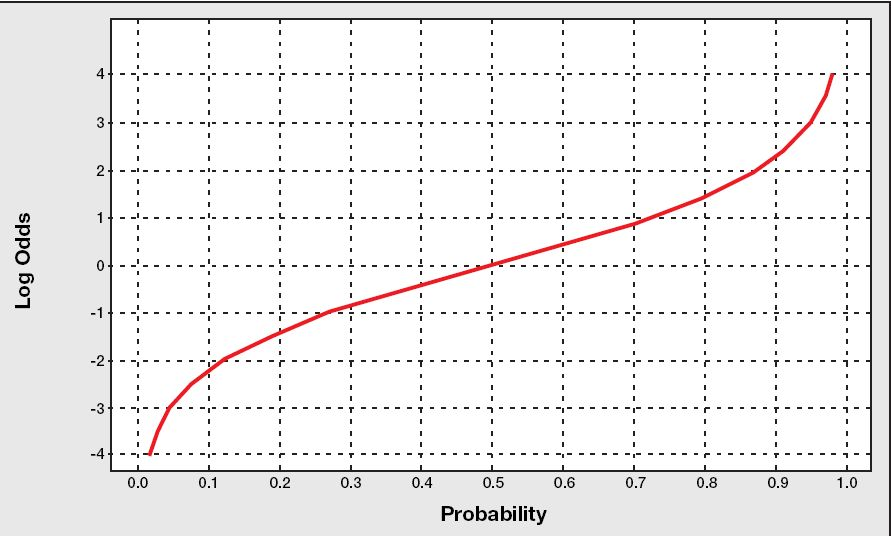
\includegraphics[scale=.33]{LogOdds}
\label{logoddsimg}
\caption{Log odds mapning.}
\end{figure}

Effekten ved at beregne forholdet mellem $x$ og $\neg x$ er den afbildning der fåes; værdierne tilordner sig efter samme skala som kendes fra decibel skalaen til måling af lydintensitet -- enhver forøgelse af 10dB giver en tifold forøgelse af den faktiske intensitet.
Sagt på en anden måde, så svarer en sandsynlighed på 50\% til 0dB, hvor symmetrien imellem dem afspejles ved negative værdier, fx er 99\% ca. 20dB, hvor 1\% svarer ca. til -20dB.

En anden umiddelbar fordel er, at forskellene bliver forstærket hvor de betyder mest.
Oversætter vi værdierne 50.00\% og 50.01\% får vi henholdsvis 0dB og 0.0017dB, hvorimod 99.98\% og 99.99\% bliver til 37dB og 40dB. \\ \\
\cite[s. 2]{logodds} \\

Ønsker vi at genskabe vores \textit{belief} udfra log odds ($l_x$), kan vi benytte følgende ligning:

\begin{equation}
bel_t(x) = 1 - \frac{1}{1 + exp\{l_x\}}
\end{equation}
 \\
\cite[s. 95]{probabilisticRobotics} 

\subsubsection{Udledning af opdateringsalgoritmen}
Ved at benytte os af bayes regel, kan vi beskrive sandsynligheden for $x$ udfra sensormålinger $z$.
\begin{equation}
\begin{split}
	P(x \mid z_{1:t}) &= \frac{P(z_t \mid x, z_{1:t-1}) P(x \mid z_{1:t-1})}{P(z_t \mid z_{1:t-1})} \\
	&= \frac{P(z_t \mid x) P(x \mid z_{1:t-1})}{P(z_t \mid z_{1:t-1})}
\end{split}
\end{equation}
Vi kan nu anvende Bayes regel på modellen for sensor målinger $P(z_t \mid x)$.
\begin{equation}
P(z_t \mid x) = \frac{P(x \mid z_t) P(z_t)}{P(x)}
\end{equation}
Hvilket vi indsætter og får.
\begin{equation}
P(x \mid z_{1:t}) = \frac{P(x \mid z_t) P(z_t) P(x \mid z_{1:t-1})}{P(x) P(z_t \mid z_{1:t-1})}
\end{equation}
 \\
\cite[s. 95]{probabilisticRobotics} \\

Vi har selvfølgelig samme type udtryk for den modsatte tilstand $\neg x$.
\begin{equation}
P(\neg x \mid z_{1:t}) = \frac{P(\neg x \mid z_t) P(z_t) P(\neg x \mid z_{1:t-1})}{P(\neg x) P(z_t \mid z_{1:t-1})}
\end{equation}
Ved at dividere de to, kan vi eliminere nogle af de sandsynligheder som er svære at beregne.

\begin{equation}
\begin{split}
	\frac{P(x \mid z_{1:t-1})}{P(\neg x \mid z_{1:t-1})} 
	&= \frac{P(x \mid z_t)}{P(\neg x \mid z_t)} \frac{P(x \mid z_{1:t-1})}{P(\neg x \mid z_{1:t-1})} \frac{P(\neg x)}{P(x)} \\
	&= \frac{P(x \mid z_t)}{1-P(x \mid z_t)} \frac{P(x \mid z_{1:t-1})}{1-P(x \mid z_{1:t-1})} \frac{1-P(x)}{P(x)}
\end{split}
\end{equation}

Vi beskriver log odds forholdet af vores \textit{belief} $bel_t(x)$ som $l_t(x)$. 
Log oddset for vores \textit{belief} til tiden $t$ er givet ved at tage logaritmen til ligningen. 

\begin{equation}
\begin{split}
	l_t(x) &= log\Bigg(\frac{P(x \mid z_t)}{1-P(x \mid z_t)}\Bigg) 
	+ log\Bigg(\frac{P(x \mid z_{1:t-1})}{1-P(x \mid z_{1:t-1})}\Bigg) + log\Bigg(\frac{1-P(x)}{P(x)}\Bigg) \\
	&= log\Bigg(\frac{P(x \mid z_t)}{1-P(x \mid z_t)}\Bigg) - log\Bigg(\frac{P(x)}{1-P(x)}\Bigg) + l_{t-1} 
\end{split}
\end{equation}

Her er $P(x)$ den \textit{prior} sandsynlighed for tilstanden $x$, og er med i alle opdateringer af
sandsynligheden for $x$. Den \textit{prior} sandsynlighed er også med til at definere den oprindelige
\textit{belief} før der tages højde for \textit{evidens} i form af sensormålinger.

\begin{equation}
 l_0 = log\Bigg(\frac{P(x)}{1-P(x)}\Bigg)
 \end{equation}
\cite[s. 96]{probabilisticRobotics} \\

Dette giver os den endelige algoritme for det binære bayes filter.

\subsubsection{Opdatering af celle med Bayesiansk filter}
Opdaterings-algoritmen tager \textit{log odds} for en \textit{posterior belief} $l_{t-1}$ for en celle, samt en ny sensor-måling $z_t$, hvorfra der returneres en \textit{log odds} for en ny \textit{belief}, $l_t$, for cellen.
Algoritmen, skrevet i pseudo-kode, kan ses i \cref{alg:binaerbayesfilter}.

\begin{algorithm}[h]
\textbf{BinaryBayesFilter($l_{t-1}, z_t$)} \\
\Indp $l_t = l_{t-1} + \log \frac{p(x \mid z_t)}{1-p(x \mid z_t)} - \log \frac{p(x)}{1-p(x)}$ \\
\Return{$l_t$}
\caption{Binært Baysiansk filter algoritme på log odds form, brugt til at estimere ny posterior ud fra sensormåling.}
\label{alg:binaerbayesfilter}
\end{algorithm}

Algoritmen tager prior ($l_{t-1}$), som lægges til sandsynligheden beregnet vha. log odds af sensormodellen, minus log odds for den negerede forskel 
af sandsynligheden for, om en celle er optaget eller ej. \\ \\
\cite[s. 94]{probabilisticRobotics}



